\documentclass[runningheads]{llncs}

\usepackage[T1]{fontenc}
\usepackage{graphicx}
\usepackage{amsmath}
\usepackage{booktabs}
\usepackage{hyperref}
\usepackage{subcaption}
\usepackage{algorithm}
\usepackage{algorithmic}
\begin{document}

\title{Classical Segmentation and Deep Learning Completion\\for LiDAR Point Clouds on SemanticKITTI}

\titlerunning{Classical Segmentation and DL Completion for LiDAR}

\author{Ngo Vi Viet Anh\inst{1} \and
Doan Nhat Quang\inst{1}}

\authorrunning{N. V. V. Anh et al.}

\institute{FPT School of Business \& Technology, FPT University, Vietnam\\
\email{ngovivietanh@gmail.com}}

\maketitle

\begin{abstract}
We present a two-phase pipeline for LiDAR point cloud processing on the SemanticKITTI dataset. Phase~1 performs object segmentation using a six-stage classical pipeline: noise removal, voxel downsampling, RANSAC ground plane extraction, HDBSCAN density-adaptive clustering, geometric filtering with ground-plane-relative height estimation, and heuristic bounding-box classification, followed by multi-frame centroid-based tracking via the Hungarian algorithm. Phase~2 addresses point cloud completion using a Point Completion Network (PCN) trained on ShapeNet, targeting the synthetic-to-real domain gap for LiDAR objects. We evaluate Phase~1 segmentation against SemanticKITTI ground truth using IoU-based precision, recall, and F1 metrics. PCN training on 3{,}834 ShapeNet vehicle models achieves a validation F-Score of 0.841 after 100 epochs. This report covers the full project from initial development through current status, including implementation details, experimental results, and planned next steps.

\keywords{LiDAR \and point cloud segmentation \and point cloud completion \and SemanticKITTI \and HDBSCAN \and PCN}
\end{abstract}


\section{Introduction}

Autonomous driving systems rely on LiDAR sensors to perceive the 3D environment. Raw LiDAR scans produce large, unstructured point clouds that must be processed to identify objects such as vehicles, pedestrians, and infrastructure. While deep learning approaches dominate current benchmarks, they require extensive labelled data and often lack interpretability. Classical methods based on geometric reasoning offer transparency and do not require training data for the segmentation stage, but struggle with the sparsity and occlusion inherent to single-scan LiDAR.

This work investigates a hybrid approach: a classical pipeline for object segmentation (Phase~1) paired with a learned point cloud completion network (Phase~2). The segmentation pipeline extracts individual objects from raw LiDAR frames without any training. The completion network, trained on synthetic ShapeNet~\cite{shapenet2015} data, reconstructs dense object shapes from the sparse partial observations produced by Phase~1. The key research question is whether this two-phase design can bridge the synthetic-to-real domain gap, using classical segmentation to provide training signal for completion and completion to enhance sparse detections.

We evaluate on SemanticKITTI~\cite{behley2019iccv}, a large-scale dataset built on the KITTI Vision Benchmark~\cite{geiger2012cvpr} with per-point semantic and instance annotations across 22 driving sequences.


\section{Related Work}

\subsection{LiDAR Point Cloud Segmentation}

Traditional LiDAR segmentation relies on geometric primitives: ground plane fitting via RANSAC~\cite{geiger2012cvpr}, followed by Euclidean or density-based clustering (DBSCAN, HDBSCAN) on the remaining points. These methods require no training data but are sensitive to parameter tuning and struggle with varying point density at different ranges.

Deep learning approaches such as PointNet, PointNet++, and RandLA-Net operate directly on point clouds, while projection-based methods (SqueezeSeg, RangeNet++) convert 3D points to 2D range images for efficient convolution. Transformer-based architectures have recently achieved state-of-the-art results on SemanticKITTI benchmarks.

\subsection{Point Cloud Completion}

Point cloud completion reconstructs dense shapes from partial observations. PCN (Point Completion Network)~\cite{yuan2018pcn} introduced a coarse-to-fine architecture with a PointNet encoder and grid-folding decoder. Subsequent works (TopNet, MSN, PoinTr, SeedFormer, SnowflakeNet) improve completion quality through attention mechanisms, seed generation, and progressive refinement.

A persistent challenge is the synthetic-to-real domain gap: models trained on clean ShapeNet meshes often degrade when applied to noisy, sparse LiDAR scans. Strategies to address this include noise augmentation during training and fine-tuning on real data.


\section{Methodology}

Our pipeline processes each LiDAR frame through six sequential stages for segmentation, applies multi-frame tracking, and then performs point cloud completion on the tracked objects. Fig.~\ref{fig:pipeline} shows the full architecture.

\begin{figure}[H]
\centering
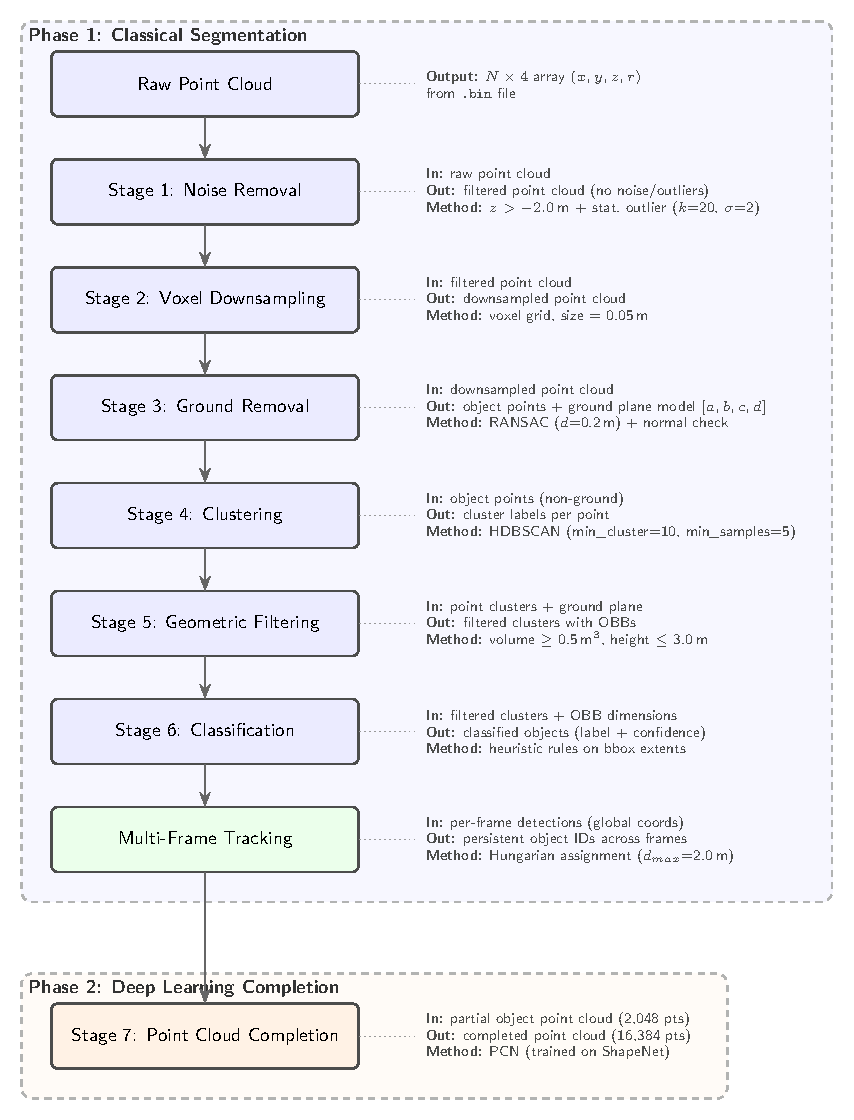
\includegraphics[width=\textwidth, height=0.85\textheight, keepaspectratio]{figures/pipeline_diagram.pdf}
\caption{Two-phase pipeline architecture. Phase~1 (blue/green) performs classical segmentation and tracking. Phase~2 (orange) applies deep learning completion.}
\label{fig:pipeline}
\end{figure}

\subsection{Phase 1: Classical Segmentation Pipeline}

\subsubsection{Stage 1: Noise Removal.}
Raw point clouds are loaded from binary files as $N \times 4$ arrays $(x, y, z, r)$ where $r$ is reflectance. Points below $z = -2.0$\,m (below the road surface) are removed. Statistical outlier removal with $k = 20$ neighbours and $\sigma = 2.0$ eliminates isolated noise points.

\subsubsection{Stage 2: Voxel Downsampling.}
The filtered cloud is downsampled using a voxel grid with cell size 0.05\,m, reducing point count while preserving spatial structure.

\subsubsection{Stage 3: Ground Plane Removal.}
RANSAC fits a plane model $ax + by + cz + d = 0$ with distance threshold 0.2\,m. A normal direction check rejects non-horizontal surfaces (walls, building facades) by requiring $|c| / \|\mathbf{n}\| > 0.5$. Ground inliers are separated from object points.

\subsubsection{Stage 4: Clustering.}
Non-ground points are clustered using HDBSCAN with \texttt{min\_cluster\_size}$\,= 10$ and \texttt{min\_samples}$\,= 5$. HDBSCAN adapts to varying point density across the scan, unlike fixed-radius DBSCAN which requires a single $\varepsilon$ that cannot simultaneously handle dense nearby and sparse distant regions. We use the dedicated \texttt{hdbscan} Python package, which is 7.7$\times$ faster than scikit-learn's implementation (0.48\,s vs 3.72\,s per frame on ${\sim}45$k points).

\subsubsection{Stage 5: Geometric Filtering.}
Each cluster's oriented bounding box (OBB) is computed. Clusters are rejected based on:
\begin{itemize}
    \item Minimum point count: $< 15$ points
    \item Volume: $< 0.5$\,m$^3$ or $> 100$\,m$^3$
    \item Maximum dimension: $> 8.0$\,m
    \item Minimum extent: max dimension $< 0.5$\,m or median dimension $< 0.2$\,m
    \item Height above ground: signed distance from OBB centre to the RANSAC plane $> 3.0$\,m
\end{itemize}

The ground-plane-relative height computation uses the signed point-to-plane distance:
\begin{equation}
h = \frac{a \cdot c_x + b \cdot c_y + c \cdot c_z + d}{\sqrt{a^2 + b^2 + c^2}}
\end{equation}
where $(c_x, c_y, c_z)$ is the OBB centre and $(a, b, c, d)$ are the RANSAC plane coefficients. This is robust to sloped terrain, unlike raw $z$-coordinate thresholds.

\subsubsection{Stage 6: Heuristic Classification.}
Filtered clusters are classified by OBB dimensions using hand-crafted rules:
\begin{itemize}
    \item \textbf{Traffic sign}: $\min < 0.15$\,m, $\max < 3.0$\,m, elevated ($z > 0.5$\,m)
    \item \textbf{Pedestrian}: $\max < 2.0$\,m, $\text{med} < 1.0$\,m, $\min < 0.8$\,m
    \item \textbf{Car}: $3.0 \leq \max \leq 5.5$\,m, $1.5 \leq \text{med} \leq 2.5$\,m
    \item \textbf{Truck}: $\max > 5.5$\,m or ($\max > 4.0$\,m and $\text{med} > 2.0$\,m)
    \item \textbf{Vegetation}: $\max > 2.0$\,m, $\min > 0.3$\,m, $\text{med} > 0.5$\,m
\end{itemize}

\subsubsection{Multi-Frame Tracking.}
Detected objects are transformed to a global coordinate frame using $\mathbf{T}_{\text{total}} = \mathbf{P}_i \cdot \mathbf{T}_r$, where $\mathbf{P}_i$ is the ego-motion pose (camera frame) and $\mathbf{T}_r$ is the LiDAR-to-camera calibration transform. A centroid-based tracker uses the Hungarian algorithm to match detections across frames with a maximum association distance of 2.0\,m. Tracks persist for up to 5 frames without a match before deletion.


\subsection{Phase 2: Point Cloud Completion}

\subsubsection{PCN Architecture.}
We implement PCN~\cite{yuan2018pcn} with the following architecture:

\paragraph{Encoder.} A stacked PointNet processes input partial point clouds $(B, N, 3)$. Stage~1 applies shared MLPs (Conv1d: $3 \to 128 \to 256$) with batch normalisation and ReLU, followed by max pooling to obtain a 256-d global feature. This feature is concatenated back to per-point features, and Stage~2 applies Conv1d $512 \to 512 \to 1024$ with max pooling, yielding a 1024-d global descriptor.

\paragraph{Decoder.} The coarse stage maps the 1024-d feature through fully connected layers ($1024 \to 1024 \to 1024 \to 3072$) to produce 1{,}024 seed points. The fine stage tiles a $4 \times 4$ 2D grid ($[-0.05, 0.05]^2$) around each seed, concatenates the grid coordinates and global feature, and applies a folding MLP (Conv1d: $1029 \to 512 \to 512 \to 3$) to predict residual offsets. The output is $1{,}024 \times 16 = 16{,}384$ fine points.

\subsubsection{Loss Function.}
The training loss combines Chamfer Distance (CD) at both levels:
\begin{equation}
\mathcal{L} = \text{CD}(\mathbf{Y}_{\text{coarse}}, \hat{\mathbf{Y}}_{\text{coarse}}) + \alpha \cdot \text{CD}(\mathbf{Y}_{\text{fine}}, \hat{\mathbf{Y}}_{\text{fine}})
\end{equation}
where $\alpha = 0.5$. The bidirectional Chamfer Distance is:
\begin{equation}
\text{CD}(\mathbf{P}, \mathbf{Q}) = \frac{1}{|\mathbf{P}|}\sum_{p \in \mathbf{P}} \min_{q \in \mathbf{Q}} \|p - q\|^2 + \frac{1}{|\mathbf{Q}|}\sum_{q \in \mathbf{Q}} \min_{p \in \mathbf{P}} \|q - p\|^2
\end{equation}

To fit within 8\,GB VRAM (RTX 3070 Ti), we use a chunked implementation that processes distance matrices in blocks of 2{,}048 columns, and subsample both predictions and ground truth to 4{,}096 points for the fine-level loss.

\subsubsection{Training Data.}
Training uses ShapeNet~\cite{shapenet2015} meshes from three KITTI-relevant categories: car (3{,}533 models), bus (939), and motorcycle (337) --- 4{,}809 models total, split 80/20 for train/val. Each mesh is scaled to real-world dimensions (car: 4.5\,m, bus: 10\,m, motorcycle: 2.2\,m) and sampled to 16{,}384 ground truth points. Partial inputs (2{,}048 points) are generated via depth-image back-projection using Open3D's \texttt{RaycastingScene}: a virtual depth camera ($256 \times 256$) renders the mesh from random viewpoints (elevation $[-20^{\circ}, 30^{\circ}]$, azimuth $[0^{\circ}, 360^{\circ}]$, radius $[2.5, 4.5]$\,m), and visible surface points are back-projected to 3D.


\section{Experiments}

\subsection{Segmentation Evaluation}

We evaluate Phase~1 against SemanticKITTI ground truth instance labels for ``thing'' classes (cars, pedestrians, cyclists, etc.). For each frame, detection masks and GT instance masks are compared using point-level IoU. Greedy matching pairs detections to GT instances by descending IoU; a match requires IoU $\geq 0.3$.

\paragraph{Metrics.}
\begin{itemize}
    \item \textbf{Precision}: fraction of detected clusters matching a GT instance
    \item \textbf{Recall}: fraction of GT instances matched by a detection
    \item \textbf{F1}: harmonic mean of precision and recall
    \item \textbf{Mean IoU}: average IoU over matched pairs
\end{itemize}

\paragraph{DBSCAN vs HDBSCAN.} Table~\ref{tab:seg_eval} compares the two clustering methods on 20 frames of sequence 00 (IoU $\geq$ 0.3).

\begin{table}[H]
\caption{Segmentation results on SemanticKITTI seq 00 (20 frames, IoU $\geq$ 0.3).}\label{tab:seg_eval}
\centering
\begin{tabular}{lccc}
\toprule
Method & Precision & Recall & F1 \\
\midrule
DBSCAN ($\varepsilon = 0.5$) & 0.188 & 0.804 & 0.305 \\
HDBSCAN & 0.154 & 0.868 & 0.261 \\
\bottomrule
\end{tabular}
\end{table}

HDBSCAN improves recall by 6.4 percentage points, detecting more GT instances due to its density-adaptive nature. However, precision drops because the adaptive algorithm also produces more small clusters that do not match any GT object. The net F1 decreases, indicating that geometric filters must be tightened to suppress false positives introduced by HDBSCAN's finer clustering.


\subsection{PCN Training Results}

PCN was trained for 100 epochs on 3{,}834 ShapeNet training samples (batch size 8, Adam optimiser, initial learning rate $10^{-4}$ with step decay $\times 0.5$ every 40 epochs). Training took approximately 18 hours on an NVIDIA RTX 3070 Ti. Table~\ref{tab:pcn_train} shows the training progression.

\begin{table}[H]
\caption{PCN training progression on ShapeNet (car/bus/motorcycle).}\label{tab:pcn_train}
\centering
\begin{tabular}{rcccccc}
\toprule
Epoch & Train Loss & Val Loss & CD Coarse & CD Fine & F-Score & LR \\
\midrule
1   & 0.672 & 0.586 & 0.396 & 0.380 & ---   & $10^{-4}$ \\
10  & 0.463 & 0.448 & 0.317 & 0.261 & 0.748 & $10^{-4}$ \\
40  & 0.403 & 0.400 & 0.287 & 0.225 & 0.809 & $5 \times 10^{-5}$ \\
80  & 0.380 & 0.374 & 0.270 & 0.209 & 0.839 & $2.5 \times 10^{-5}$ \\
100 & 0.371 & 0.375 & 0.270 & 0.210 & 0.841 & $2.5 \times 10^{-5}$ \\
\bottomrule
\end{tabular}
\end{table}

The best checkpoint by validation loss occurs at epoch 80 (val loss 0.374, F-Score 0.839). Loss converges around epoch 60--70, with the final 30 epochs providing minimal improvement. Each learning rate reduction yields a small but measurable gain. The F-Score of 0.841 indicates that the model reconstructs ShapeNet vehicle shapes at reasonable quality, though this is measured on clean synthetic data.


\section{Discussion}

\subsection{Segmentation Analysis}

The current segmentation pipeline achieves high recall (0.868 with HDBSCAN) but low precision (0.154), indicating significant over-segmentation. The primary sources of false positives are:
\begin{itemize}
    \item Tree canopies and vegetation clusters that pass geometric filters
    \item Building fragments and wall sections not rejected by the ground-plane normal check
    \item Small noise clusters that exceed the minimum volume threshold
\end{itemize}

Potential improvements include aspect-ratio filtering, compactness metrics, and raising the minimum point count per cluster.

\subsection{Completion: Synthetic-to-Real Gap}

PCN training on ShapeNet shows promising in-domain results (F-Score 0.841), but the critical test is application to real KITTI LiDAR objects, which exhibit:
\begin{itemize}
    \item Higher noise levels than synthetic depth rendering
    \item Sparser point distributions, especially at long range
    \item Occlusion patterns from other objects (not just self-occlusion)
    \item Scale and orientation variations not present in normalised ShapeNet models
\end{itemize}

Domain adaptation strategies under consideration include noise augmentation during training (\texttt{simulate\_lidar\_noise}), fine-tuning on real sparse/dense pairs extracted from multi-frame accumulation, and Earth Mover's Distance (EMD) loss for the coarse output.

\subsection{Pipeline Integration Status}

Phase~1 is fully operational: the six-stage pipeline processes raw LiDAR frames, tracks objects across frames, and outputs classified bounding boxes with persistent IDs. Phase~2 (completion) has a trained model but is not yet integrated into the live pipeline. The completion model has been trained and evaluated on synthetic data only; real-world evaluation on KITTI objects is the immediate next step.


\section{Next Steps}

\begin{enumerate}
    \item \textbf{Qualitative PCN evaluation.} Visualise completions on ShapeNet test samples (input $\to$ coarse $\to$ fine) to assess reconstruction quality beyond aggregate metrics.
    \item \textbf{KITTI domain transfer.} Run the trained PCN on real partial point clouds extracted by the segmentation pipeline --- the key experiment for validating the two-phase approach.
    \item \textbf{Geometric filter tuning.} Tighten filters (aspect ratio, compactness, minimum points) to reduce HDBSCAN false positives and improve precision.
    \item \textbf{EMD loss.} Add Sinkhorn-approximated Earth Mover's Distance for the coarse output to improve point distribution uniformity.
    \item \textbf{Domain adaptation.} Fine-tune PCN with sim-to-real noise augmentation and real KITTI sparse/dense pairs from multi-frame tracking.
    \item \textbf{Stronger architectures.} Evaluate PoinTr or SeedFormer if PCN quality is insufficient on real data.
\end{enumerate}


\begin{credits}
\subsubsection{\ackname}
This work is conducted as part of the Master's thesis programme at FPT School of Business \& Technology, FPT University.

\subsubsection{\discintname}
The authors have no competing interests to declare that are relevant to the content of this article.
\end{credits}

\bibliographystyle{splncs04}
\bibliography{../references}

\end{document}
